%%%%%%%%%%%%%%%%%%%%%%%%%%%%%%%%%%%%%%%%%
% Short Sectioned Assignment
% LaTeX Template
% Version 1.0 (5/5/12)
%
% This template has been downloaded from:
% http://www.LaTeXTemplates.com
%
% Original author:
% Frits Wenneker (http://www.howtotex.com)
%
% License:
% CC BY-NC-SA 3.0 (http://creativecommons.org/licenses/by-nc-sa/3.0/)
%
%%%%%%%%%%%%%%%%%%%%%%%%%%%%%%%%%%%%%%%%%


%----------------------------------------------------------------------------------------
%	PACKAGES AND OTHER DOCUMENT CONFIGURATIONS
%----------------------------------------------------------------------------------------

\documentclass[paper=a4, fontsize=11pt]{scrartcl} % A4 paper and 11pt font size

\usepackage{float}
\usepackage{caption}
\usepackage[T1]{fontenc} % Use 8-bit encoding that has 256 glyphs
\usepackage{fourier} % Use the Adobe Utopia font for the document - comment this line to return to the LaTeX default
\usepackage[english]{babel} % English language/hyphenation
\usepackage{amsmath,amsfonts,amsthm} % Math packages

\usepackage{lipsum} % Used for inserting dummy 'Lorem ipsum' text into the template

\usepackage{sectsty} % Allows customizing section commands
\allsectionsfont{\normalfont\scshape} % Make all sections centered, the default font and small caps

\usepackage{fancyhdr} % Custom headers and footers
\pagestyle{fancyplain} % Makes all pages in the document conform to the custom headers and footers
\fancyhead{} % No page header - if you want one, create it in the same way as the footers below
\fancyfoot[L]{} % Empty left footer
\fancyfoot[C]{} % Empty center footer
\fancyfoot[R]{\thepage} % Page numbering for right footer
\renewcommand{\headrulewidth}{0pt} % Remove header underlines
\renewcommand{\footrulewidth}{0pt} % Remove footer underlines
\setlength{\headheight}{13.6pt} % Customize the height of the header


\setlength\parindent{0pt} % Removes all indentation from paragraphs - comment this line for an assignment with lots of text

\usepackage{listings}
\usepackage{paralist}
\usepackage{tikz}
\usepackage{hyperref}

\newcommand{\todo}[1]{{\huge \textcolor{red}{TODO: #1}}}
\newcommand{\ttt}[1]{{\footnotesize \texttt{#1}}}
\newcommand{\secref}[1]{\S \ref{sec:#1}}

%----------------------------------------------------------------------------------------
%	TITLE SECTION
%----------------------------------------------------------------------------------------

\newcommand{\horrule}[1]{\rule{\linewidth}{#1}} % Create horizontal rule command with 1 argument of height

\title{	
\normalfont \normalsize 
\horrule{0.5pt} \\[0.4cm] % Thin top horizontal rule
\huge CS 5220 Project 3 -- Team 6 Final Report \\ % The assignment title
\horrule{2pt} \\[0.5cm] % Thick bottom horizontal rule
}

\date{\normalsize\today} % Today's date or a custom date

\author{Taejoon Song, Junteng Jia, Joshua Cohen \\
				\{ts693, jj585, jbc264\}@cornell.edu}

\begin{document}

\graphicspath {{figs/}}
\maketitle % Print the title
\section{Introduction}\label{sec:intro}

In this project, we analyze the OpenMP version of Floyd-Warshall algorithm by profiling the code using Vtune to identify bottlenecks. The Vtune profiling result is shown in section \secref{profiling}. To tune the code, we explore different compiler flags (section \secref{compilerflags}) and slightly vectorized the code (section \secref{vectorization}). Finally we perform strong and weak scaling in section \secref{evaluation}. 
\section{Profiling}
\label{sec:profile}
%Taejoon%
\subsection{Profiling}
In order to find the bottlenecks of path, we first profiled our code
using Intel's VTune Amplifier (It was broken in cluster, so we used
it on local machine), as shown in Figure \ref{amplxe-command}.

\vspace{0.3cm}

\begin{figure}[H]
\footnotesize
\begin{verbatim}
amplxe-cl -collect advanced-hotspots ./path
amplxe-cl -report hotspots -source-object function=<NAME>
\end{verbatim}
\caption{VTune Amplifier Command}
\label{amplxe-command}
\end{figure}

\subsection{Initial Profiling Result}
Initial profile result can be found at Figure \ref{initial_profile_result_0},
and more detail in Figure \ref{initial_profile_result_1}.

We found that "square" function is the main bottleneck and do the most critical
steps for this program, so this point is where we started to tune the code.

\begin{figure}[H]
    \centering
    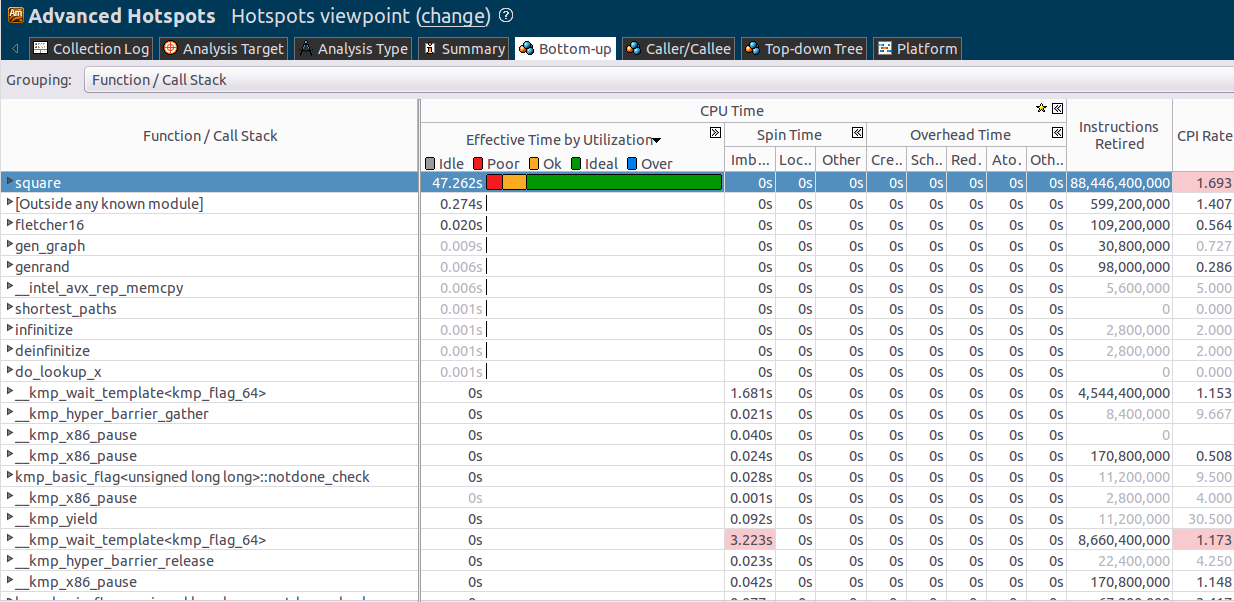
\includegraphics[width=0.65\textwidth]{figs/0_analysis.png}
    \caption{Initial Profile Analysis}
    \label{initial_profile_result_0}
\end{figure}

\begin{figure}[H]
    \centering
    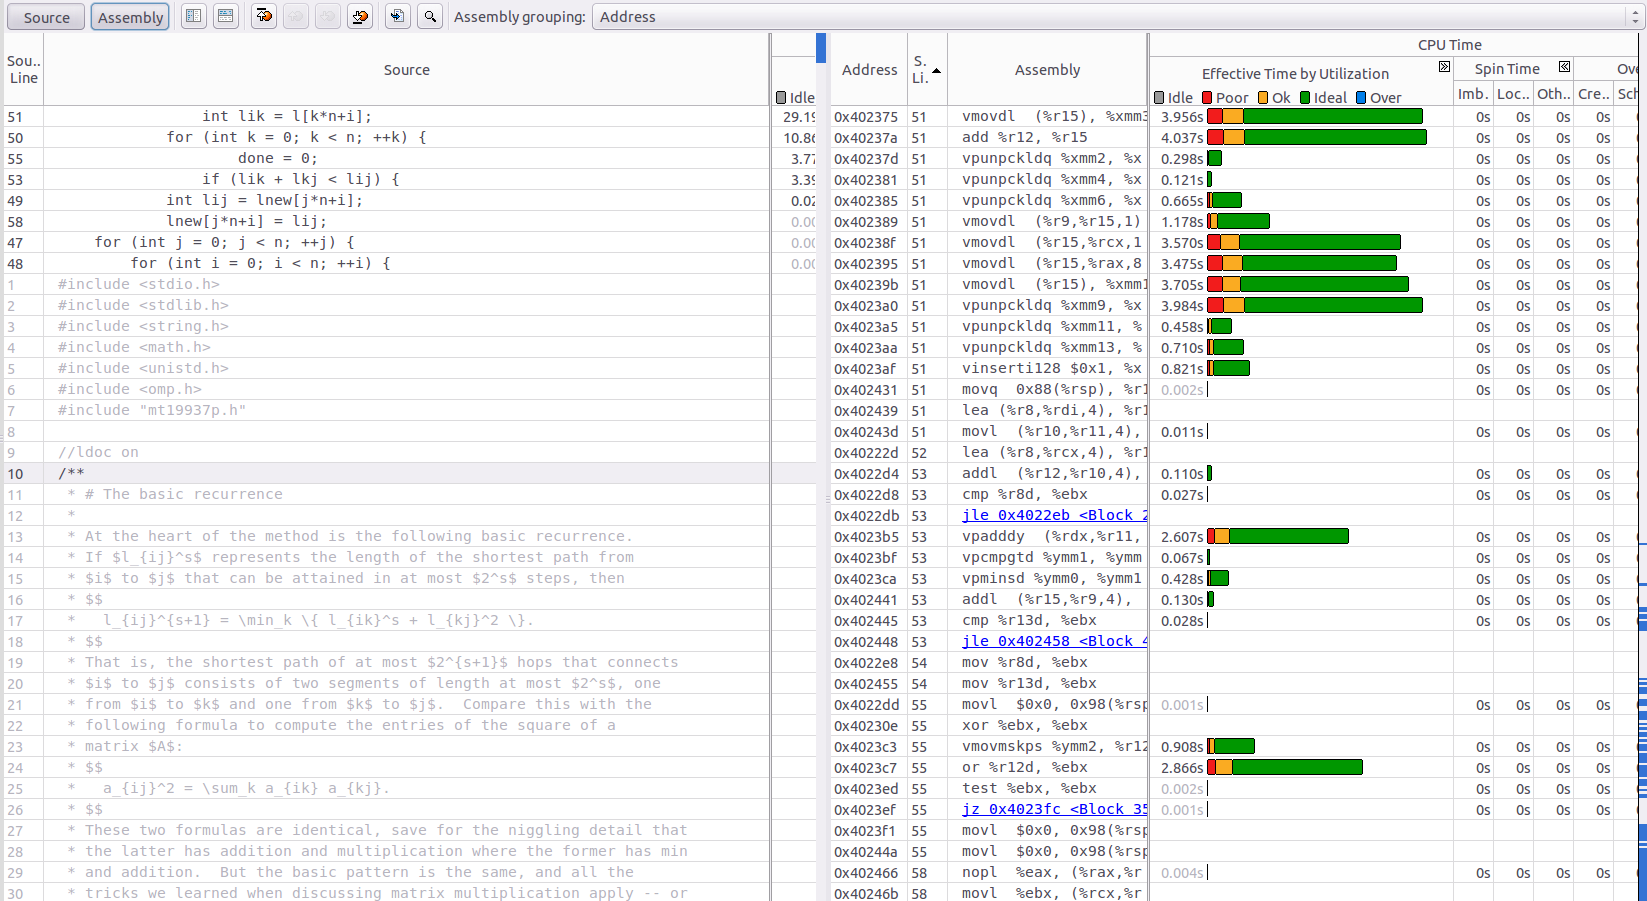
\includegraphics[width=0.65\textwidth]{figs/0_assembly.png}
    \caption{Initial Assembly Result}
    \label{initial_profile_result_1}
\end{figure}

\subsection{Initial Timing Result}

Initial timing result is shown in Figure \ref{initial_profile_result_2}. As we
can see the program is running with 8 threads using OpenMP and it takes 11.0818
seconds for 2000 vertices.

\begin{figure}[H]
    \centering
    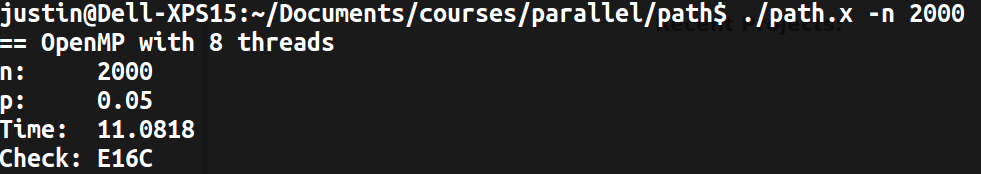
\includegraphics[width=0.8\textwidth]{figs/0_timing.png}
    \caption{Initial Timing Result}
    \label{initial_profile_result_2}
\end{figure}


\section{Vectorization}\label{sec:vector}
%Justin%
%Josh%

\subsection{Timing After Vectorization}
In order to vectorize properly vectorize our code, we looked at the output of \texttt{ipo\_out.optrpt} after compiling with flags \texttt{-qopt-report=5 -qopt-report-phase=vec}. We first were able to vectorize our call to \texttt{square} within \texttt{shortest\_paths} within \texttt{path.c} by explicitly precomputing the transpose of \texttt{l} during each call to \texttt{square}, and then replacing the assignment of \texttt{lik} directly from \texttt{l}, as
\begin{gather*}
\texttt{int lik = l[k*n+i]}
\end{gather*}
to an assignment instead from the transpose, as
\begin{gather*}
\texttt{int lik = l\_T[i*n+k]}
\end{gather*}
We also attempted to solve the issue of unaligned memory access from within \texttt{l} and \texttt{l\_T} by replacing calls to \texttt{malloc} with \texttt{\_mm\_malloc} (and, correspondingly, calls to \texttt{free} with calls to \texttt{\_mm\_free}), using a byte alignment of 32 since we're compiling with AVX2 (using the flag \texttt{-xcore-avx2}). This solved some of the issues with unaligned access, according to the vectorization report, but there are still cases with unaligned access reported.

\subsection{Timing After Vectorization}

\begin{figure}[H]
    \centering
    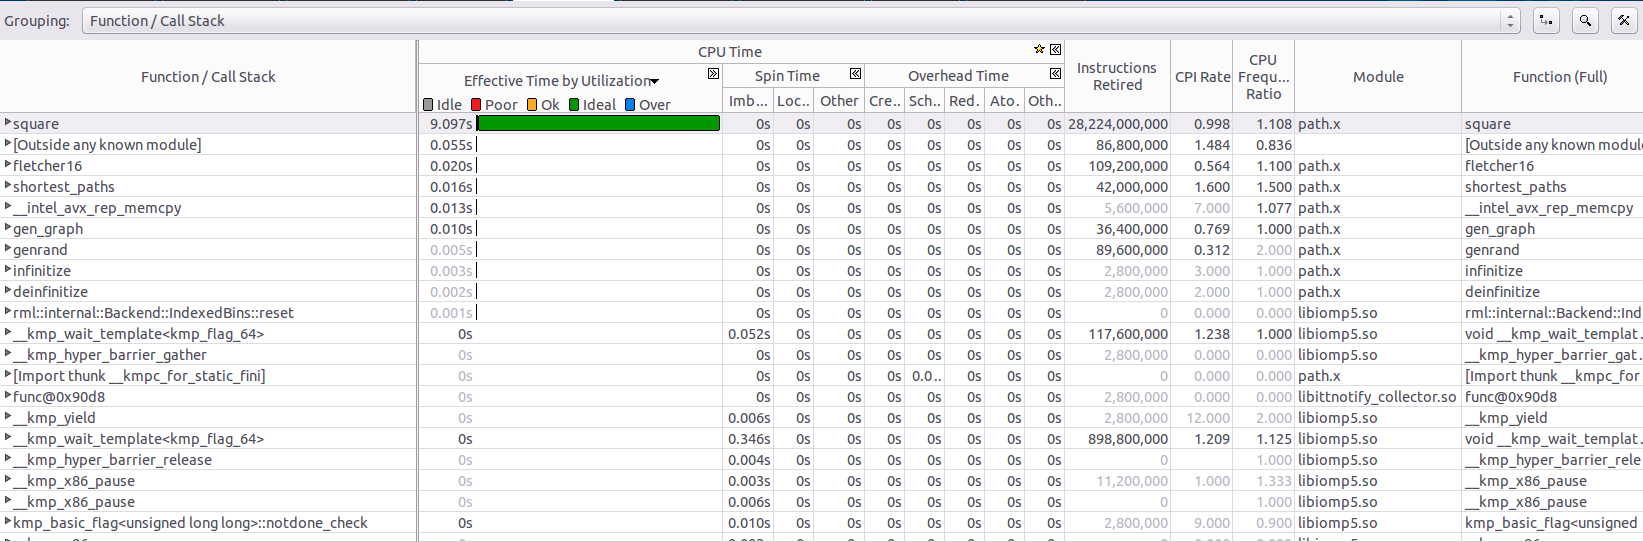
\includegraphics[width=0.8\textwidth]{figs/1_analysis.png}
    \caption{Profile Analysis After Vectorization}
    \label{vectorized_profile_result_0}
\end{figure}

As show in the picture, for the same problem size, the function \texttt{square} is more than 5
times faster than it was before, when we are running it with in Vtune, where one core is used to
trace other threads. In fact, running it with command line and time it with build in function
\texttt{omp\_get\_time()} shows the saving gives us a factor of more than 9 times faster.

\begin{figure}[H]
    \centering
    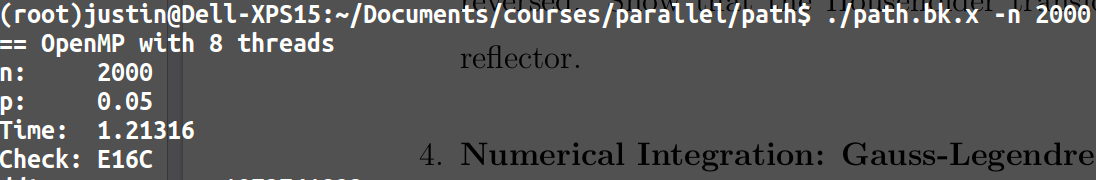
\includegraphics[width=0.8\textwidth]{figs/1_timing.png}
    \caption{Timing Result After Vectorization}
    \label{vectorized_profile_result_1}
\end{figure}

\begin{figure}[H]
    \centering
    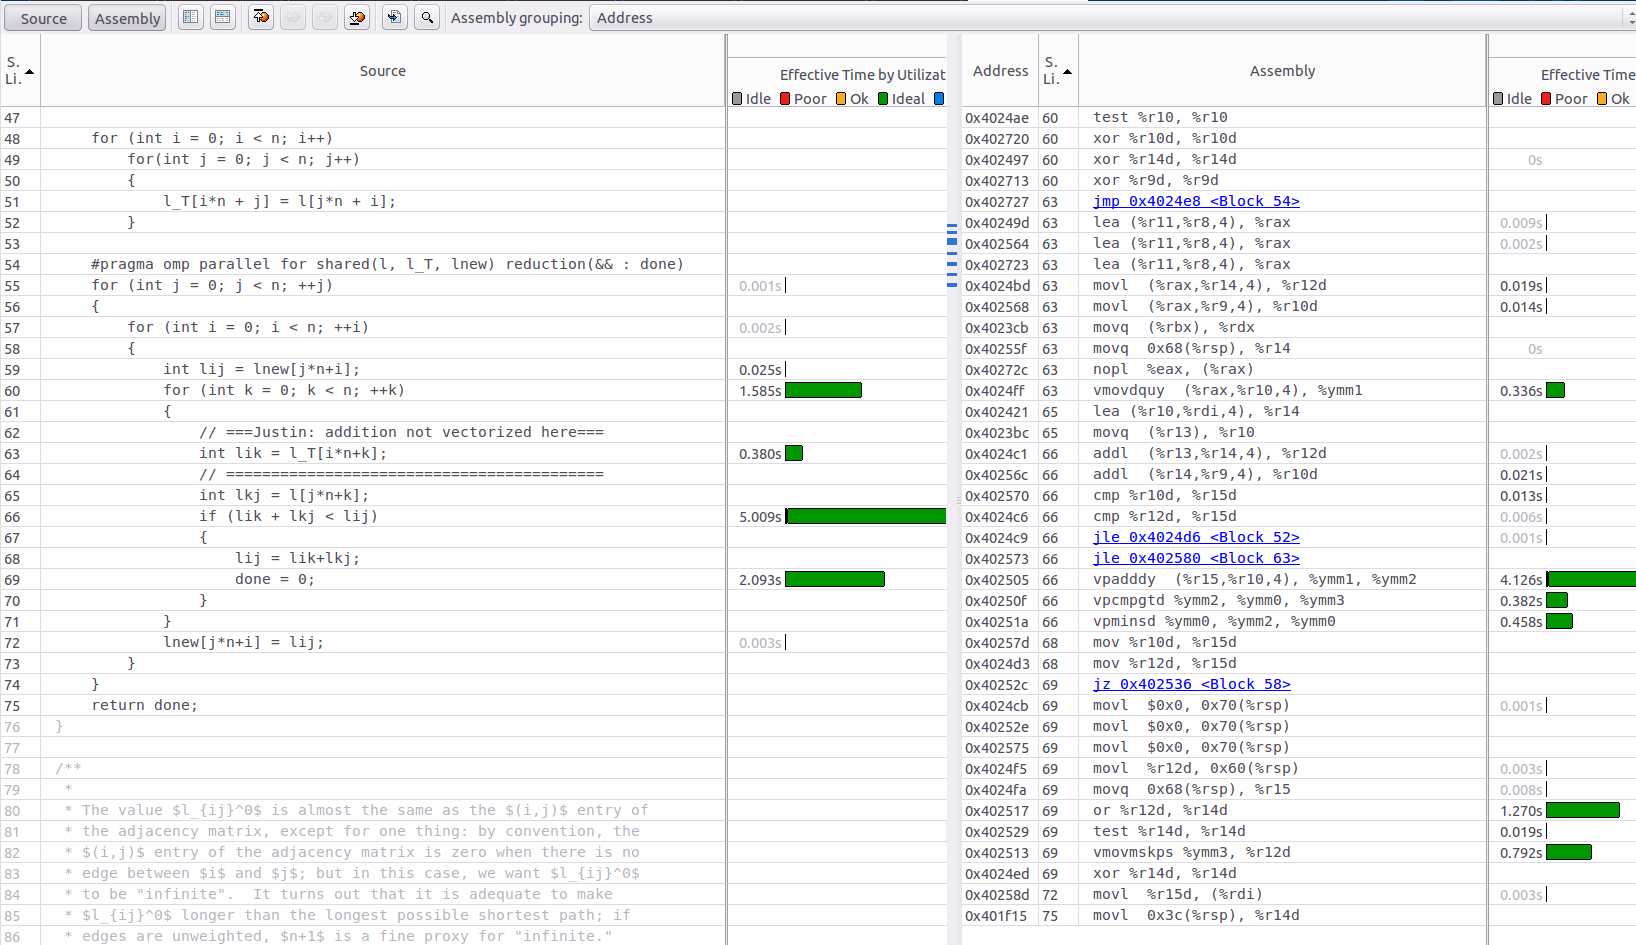
\includegraphics[width=0.8\textwidth]{figs/1_assembly.png}
    \caption{Assembly Analysis After Vectorization}
    \label{vectorized_profile_result_2}
\end{figure}

The assembly analysis is more informative as it tells how well our functions have been vectorized
as well as the timing. From the assembly analysis after vectorization, we can tell that the computations
in the inner has been vectorized. Which is where the savings come from.



\subsection{Data-Type Optimization}
As we went through tests, we found that the maximum distance between two vertices is
always below 20, even when we are calculating a 10000 by 10000 graph. Then it naturally
follows that, we don't necessarily need a 4-byte \textcolor{blue}{int} to store the
distance information. \\

To fit more data into register so that we can carry out more operation per cycle, we used
a prototype called \textcolor{blue}{ddt}, which can be any data type such as \textcolor{blue}{long},
\textcolor{blue}{short}, and \textcolor{blue}{char}. In fact, this gives us 30\% saving when we are
using \textcolor{blue}{char} to store the distance between two vertices. \\

Notice in Figure 8, we printed out a variable called \texttt{ddt\_upper\_range} which tells us the largest
distance we can have, in order to use one certain data-type. In the case with \textcolor{blue}{char}, the
largest distance is 127, which is proved to be more than enough by our tests.


\subsection{Tuned OpenMP Timing Result}

\begin{figure}[H]
    \centering
    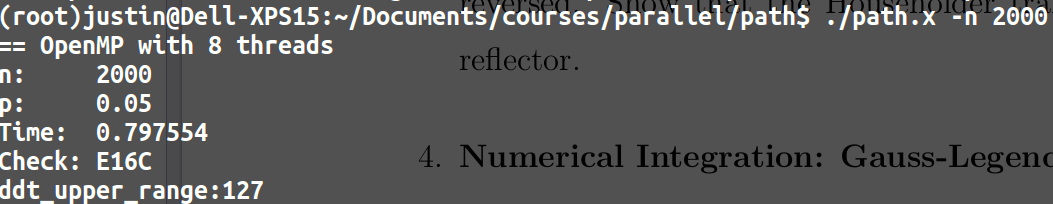
\includegraphics[width=0.8\textwidth]{figs/2_timing.png}
    \caption{Timing Result After OpenMP tuning}
    \label{ddt_profile_result_2}
\end{figure}

Timing result before introducing MPI is shown in Figure \ref{ddt_profile_result_2}.
As we can see the program is running with 8 threads using OpenMP and it takes 0.7976
seconds for 2000 vertices.

\subsection{Tuned OpenMP Profiling Result}

\begin{figure}[H]
    \centering
    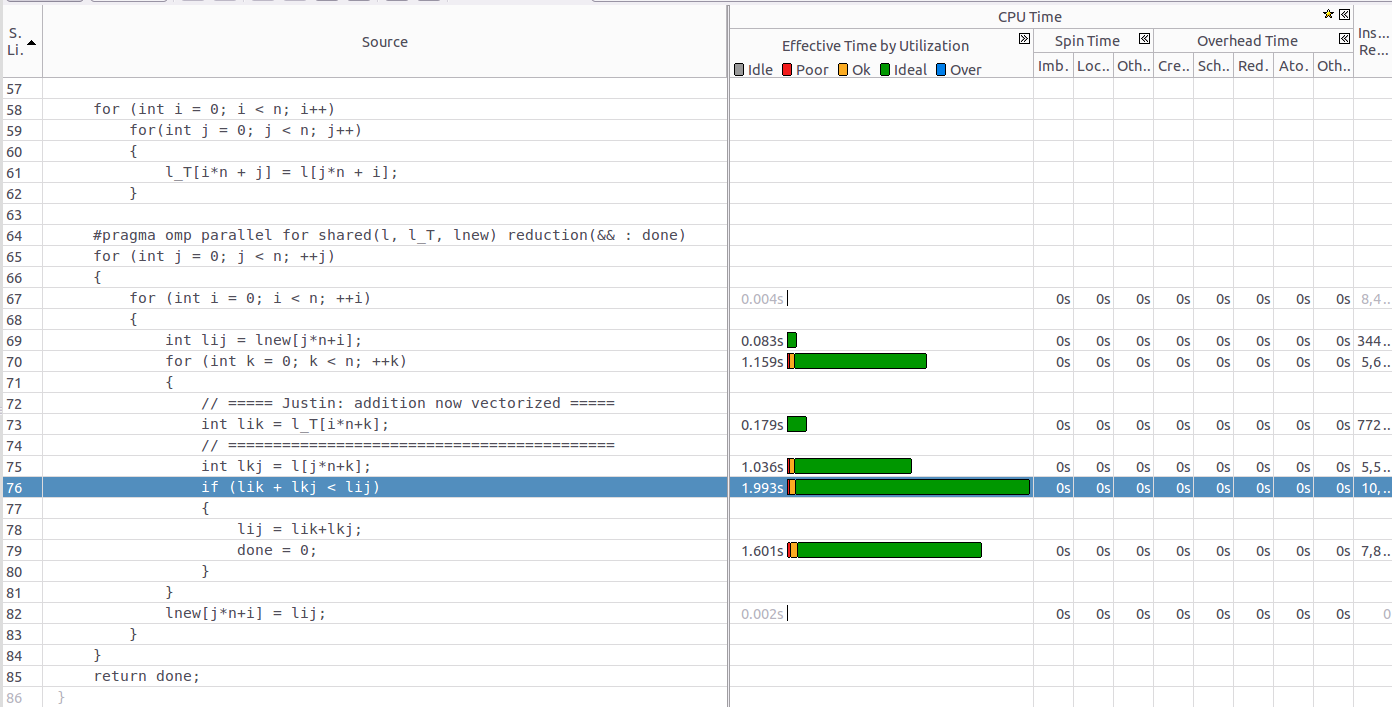
\includegraphics[width=0.8\textwidth]{figs/2_assembly.png}
    \caption{Initial Assembly Result}
    \label{ddt_profile_result_1}
\end{figure}

The assembly analysis after using data-type \textcolor{blue}{char} is down below. Comparing with Figure
\ref{vectorized_profile_result_2}, we can tell that the major saving comes from the addition between 
\texttt{lij} and \texttt{ljk}, which consist with what we would expect, since we can now fit more additions
into vector register to be calculated in one cycle.


\section{Parallelization}\label{sec:parallelization}
We parallelized the \rs{}, \block{}, and \fw{} algorithm using three
parallelization mechanisms: OpenMP, MPI, and a hybrid of the two. In this
section, we describe in detail how each mechanisms was used for parallelization.

\subsection{OpenMP}
Parallelizing each algorithm is simply a matter of using \texttt{\#pragma omp
parallel for} before each outer loop of each algorithm's respective square
functions. The implementations of this algorithm are in \texttt{rs-omp.c},
\texttt{block-omp.c}, and \texttt{fw-omp.c}.

\subsection{MPI}
Implementing the algorithms in MPI requires decomposing the problem into sub
parts, similar to the idea of domain decomposition from the last project. We
drew inspiration from previous work with distance-vector routing using
Bellman$-$Ford in determining shortest distances between routers. In that
algorithm, each router sends its distances to all other routers (each time
there is a change) to its neighbors which then use that information to update
their own distances. This continues until no routers have changed distances.

In our case we do not necessarily have a single thread per node, as there maybe
not be enough available hardware threads. Instead each ``router'' is an MPI
rank and is responsible for a set of nodes rather than a single node. Each MPI
rank calculates the minimum distance to each of its nodes from all other nodes
going through each node between 1 and $N$.

For \rs{} and \block{} each rank also determines if any distances have changed.
All MPI ranks then synchronize, to gather distances from one another and
determine if any distances have changed (if none stop then we are done and the
``master'' rank (rank 0) outputs checksum and timing information). To determine
if any distances have changed we use \texttt{mpi\_allreduce} on each rank's done
variable. To synchronize distances across all ranks we use
\texttt{mpi\_allgather} which sends each rank's distances to all other ranks and
collects them from every rank, including itself, into a single buffer. In the
case of \fw{} must synchronize for every iteration of $k$, and does not need to
check if its finished as the algorithm will always finish in the same number of
loops (N). Our implementations are in \texttt{rs-mpi.c}, \texttt{block-mpi.c},
and \texttt{fw-mpi.c}.

\subsection{Hybrid} MPI and OMP interact seamlessly when put together, making it
easy to combine our MPI implementation and the origin OMP implementation. Given
a fixed number of MPI ranks, $r$, and $p$ available threads then each MPI rank
will have access to $p/r$ threads which can be used in OMP parallel sections of
code. This can mean we do not take full advantage of all threads available to us
if $p$ is not divisible by $r$. We implemented a hybrid version of each
algorithm (by combining our MPI implementation and the OMP parts of the original
implementation) in \texttt{rs-hybrid.c}, \texttt{block-hybrid.c}, and \texttt
{fw-hybrid.c}.

\section{Evaluation}\label{sec:eval}

We evaluated our mpi, hybrid implementations of each algorithm (rs, block, fw) by doing strong scaling studies across a range of problem sizes. For rs and block we used a baseline of \rs{omp} and for fw we used a baseline of \fw{omp}. For rs and block we also did weak scaling studies for with a constant work of problem size $n=500$.

\subsection{RS}

\subsubsection{MPI}

\begin{figure}[ht]
\centering
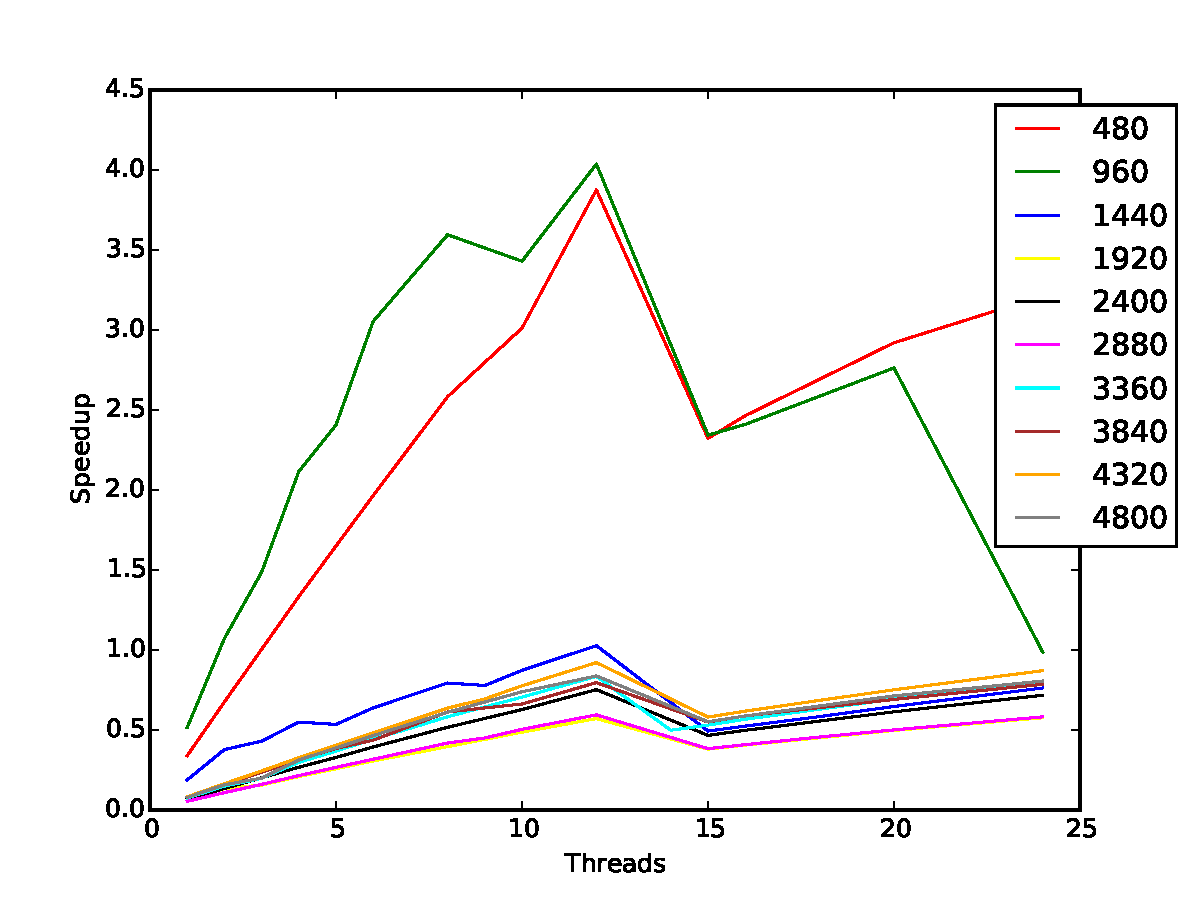
\includegraphics[width=0.5\textwidth]{plots/strong_rs-mpi_baseline-rs-omp--1.pdf}
\caption{Strong scaling for rs-mpi with a baseline of rs-omp}
\label{strong-rs-mpi}
\end{figure}

\begin{figure}[ht]
\centering
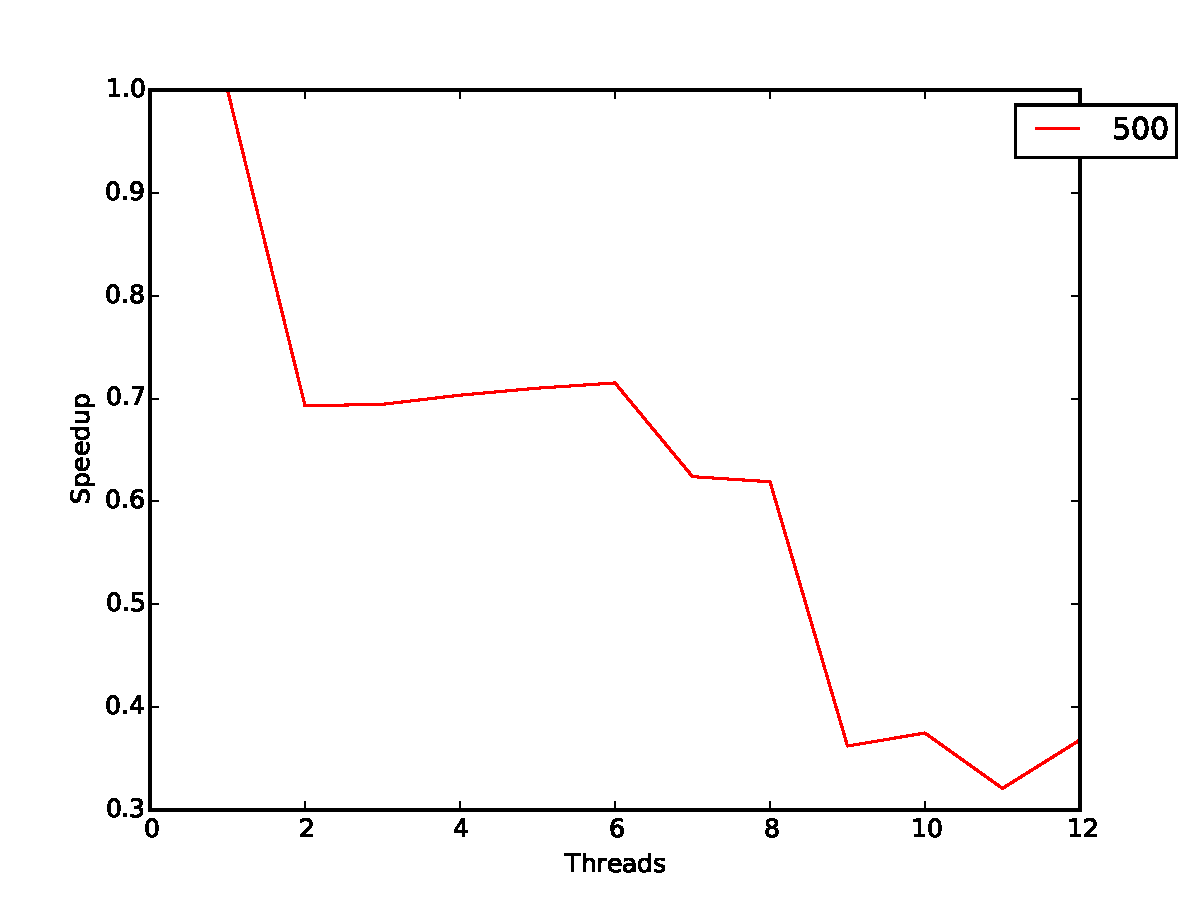
\includegraphics[width=0.5\textwidth]{plots/weak_rs-mpi.pdf}
\caption{Weak scaling for rs-mpi (baseline of itself).}
\label{weak-rs-mpi}
\end{figure}

\subsubsection{Hybrid}

\begin{figure}[ht]
\centering
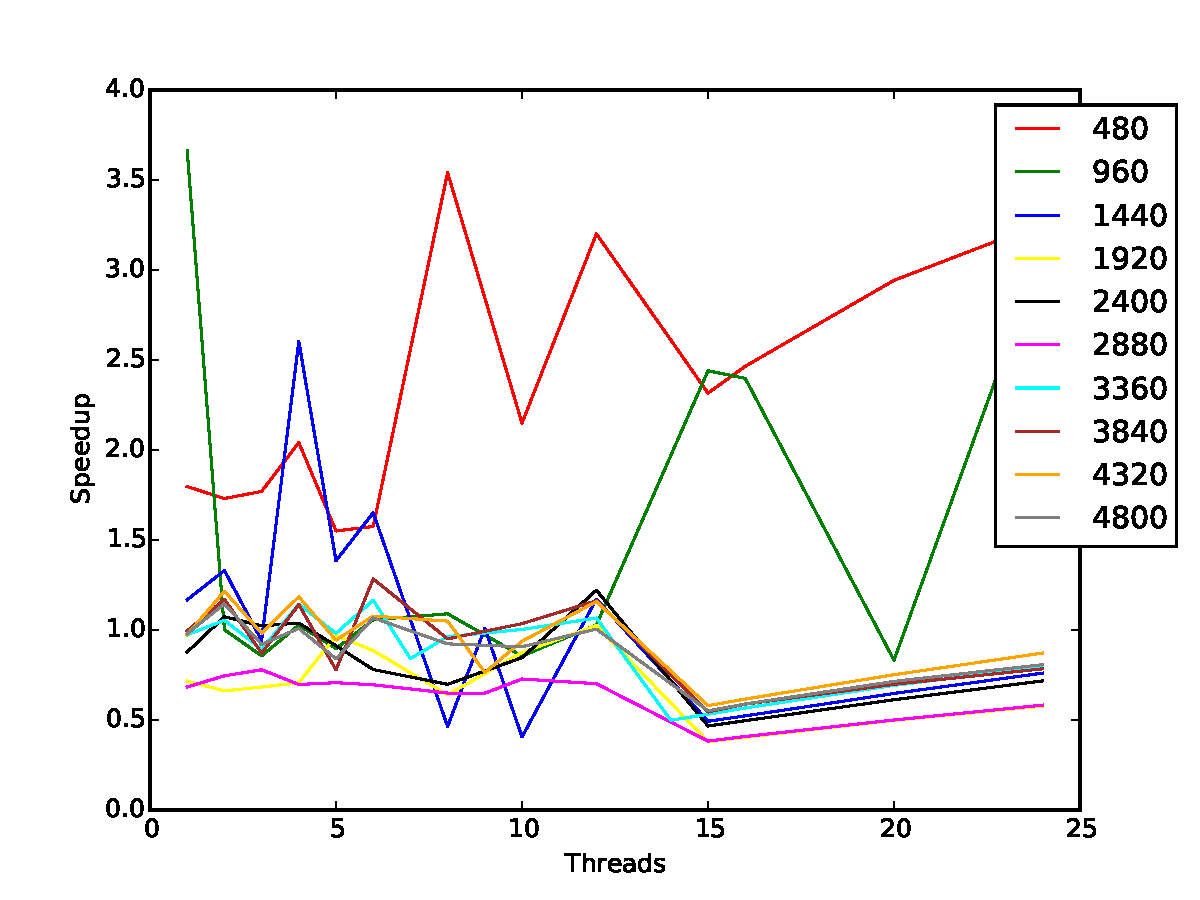
\includegraphics[width=0.5\textwidth]{plots/strong_rs-hybrid_baseline-rs-omp--1.pdf}
\caption{Strong scaling for rs-hybrid with a baseline of rs-omp}
\label{strong-rs-hybrid}
\end{figure}

\begin{figure}[ht]
\centering
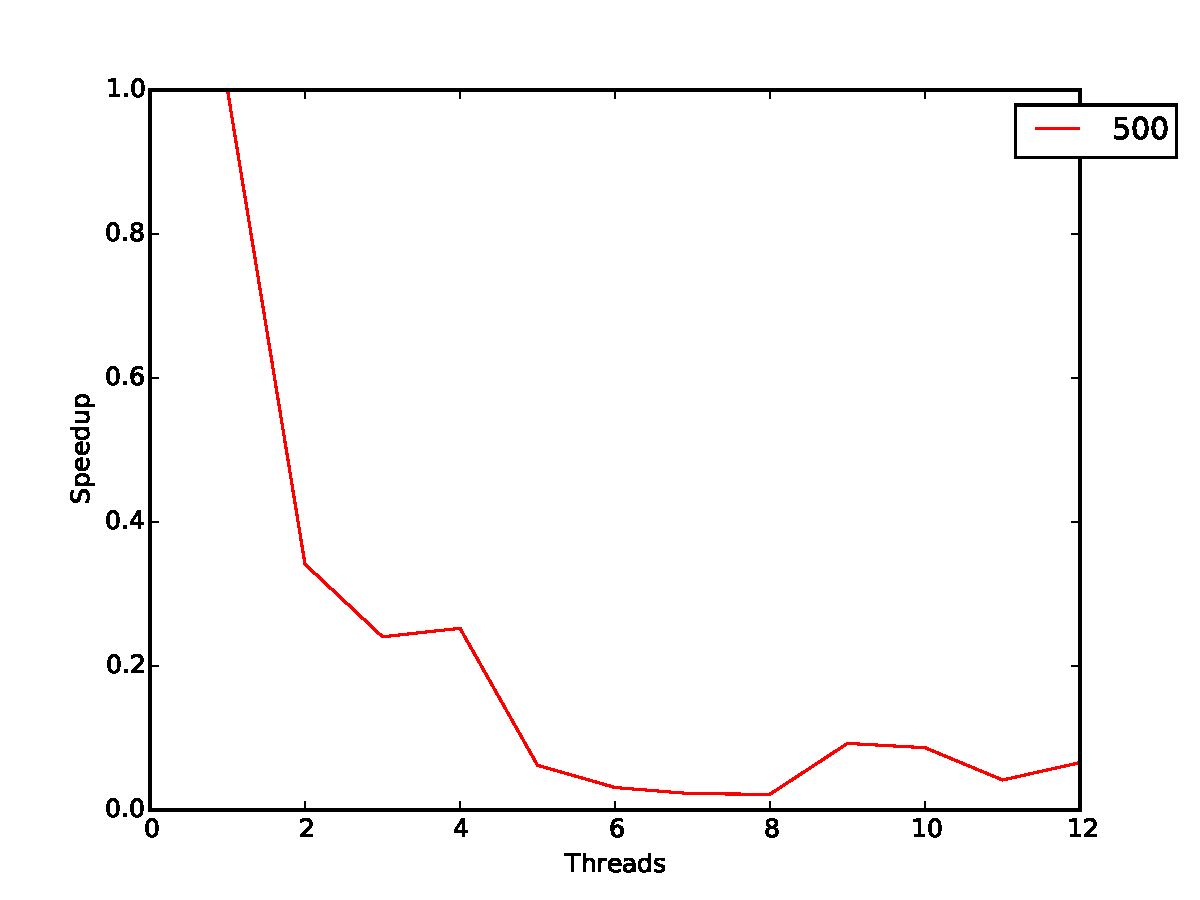
\includegraphics[width=0.5\textwidth]{plots/weak_rs-hybrid.pdf}
\caption{Weak scaling for rs-hybrid (baseline of itself).}
\label{weak-rs-hybrid}
\end{figure}


\subsection{Block}

\subsubsection{MPI}

\begin{figure}[ht]
\centering
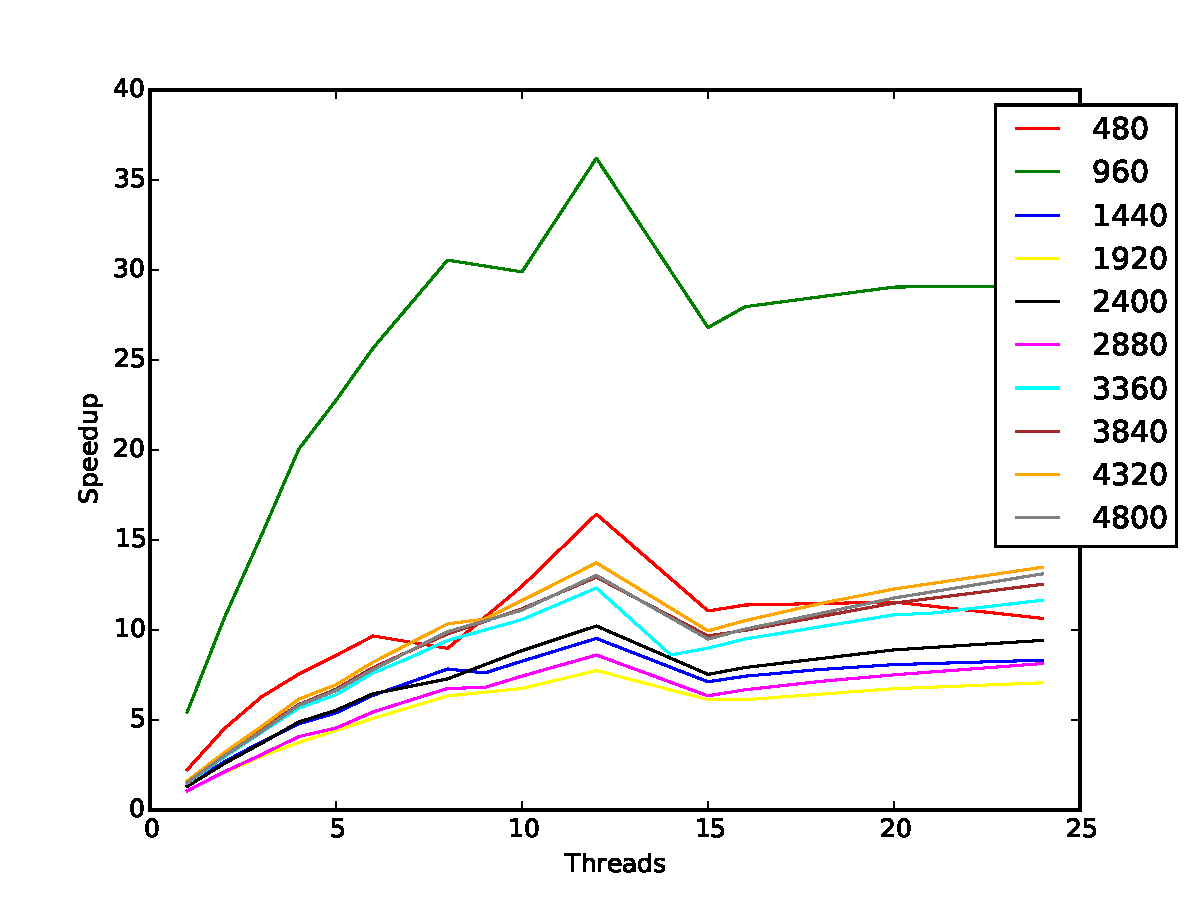
\includegraphics[width=0.5\textwidth]{plots/strong_block-mpi_baseline-rs-omp--1.pdf}
\caption{Strong scaling for block-mpi with a baseline of rs-omp}
\label{strong-block-mpi}
\end{figure}

\begin{figure}[ht]
\centering
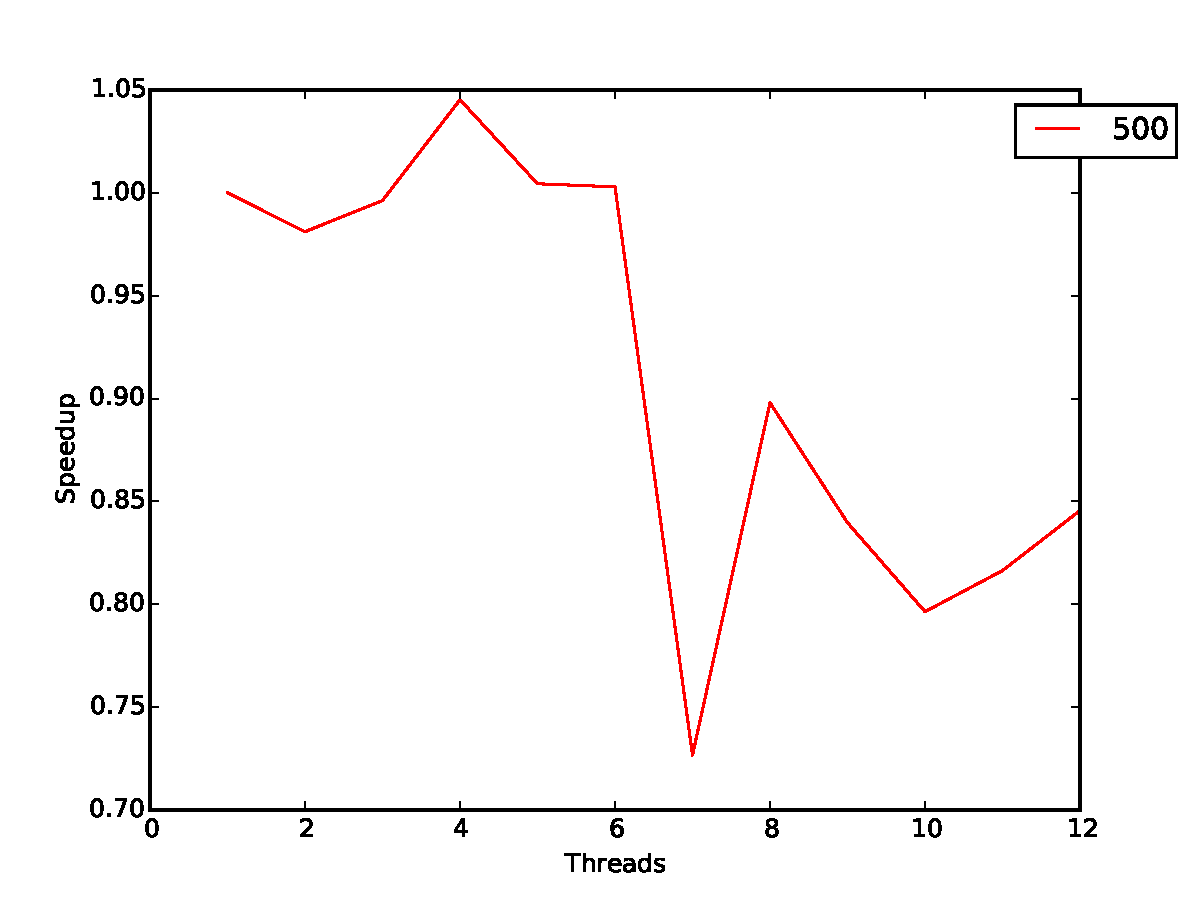
\includegraphics[width=0.5\textwidth]{plots/weak_block-mpi.pdf}
\caption{Weak scaling for block-mpi (baseline of itself).}
\label{weak-block-mpi}
\end{figure}

\subsubsection{Hybrid}

\begin{figure}[ht]
\centering
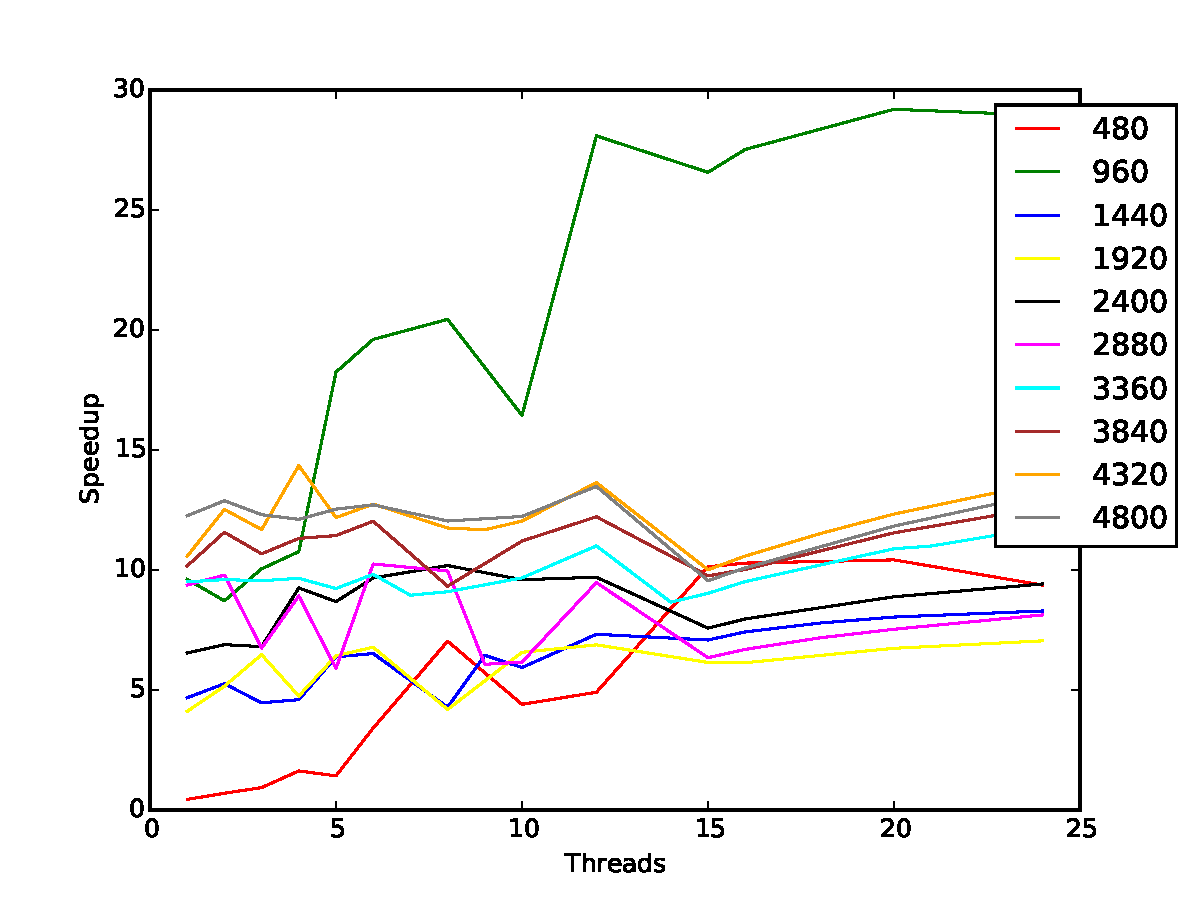
\includegraphics[width=0.5\textwidth]{plots/strong_block-hybrid_baseline-rs-omp--1.pdf}
\caption{Strong scaling for block-hybrid with a baseline of rs-omp}
\label{strong-block-hybrid}
\end{figure}

\begin{figure}[ht]
\centering
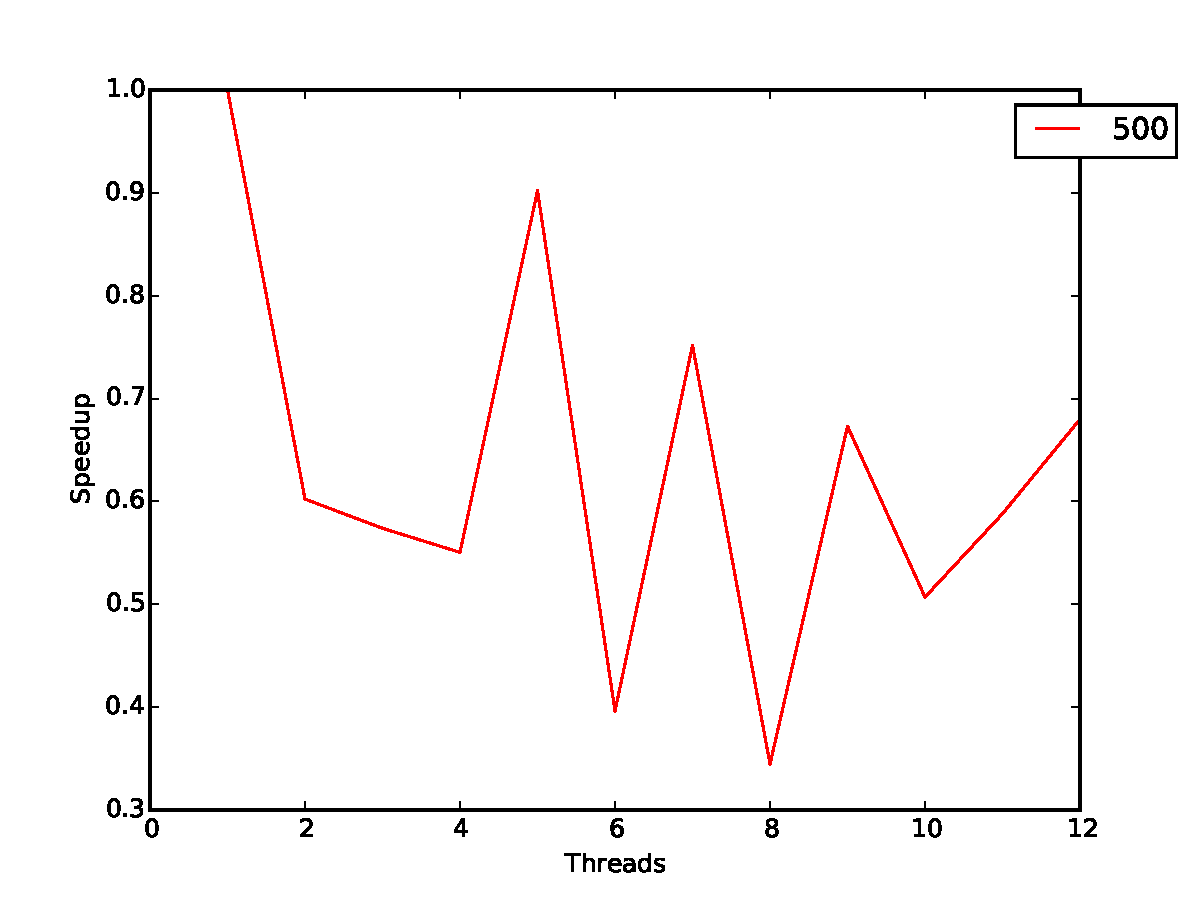
\includegraphics[width=0.5\textwidth]{plots/weak_block-hybrid.pdf}
\caption{Weak scaling for block-hybrid (baseline of itself).}
\label{weak-block-hybrid}
\end{figure}

\subsection{FW}

\subsubsection{MPI}

\begin{figure}[ht]
\centering
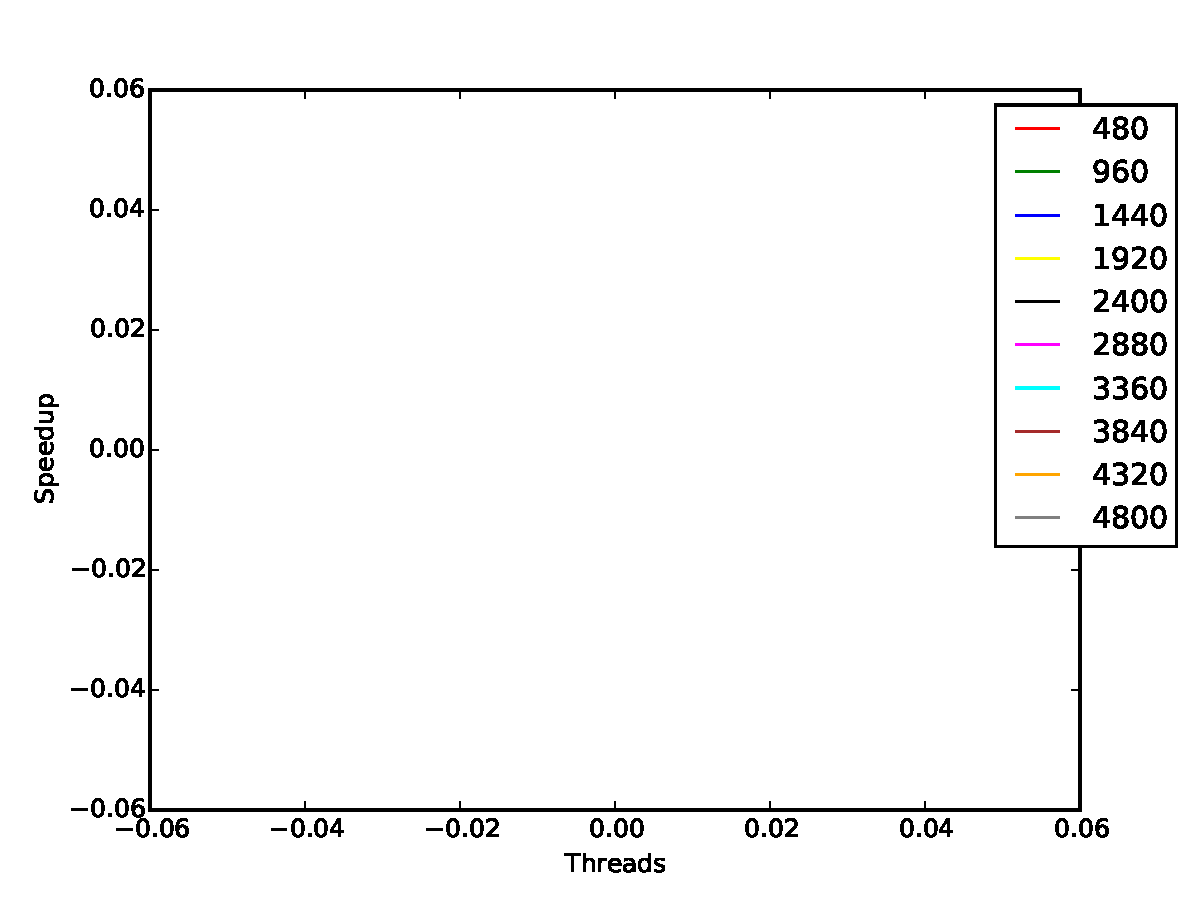
\includegraphics[width=0.5\textwidth]{plots/strong_fw-mpi_baseline-fw-omp--1.pdf}
\caption{Strong scaling for fw-mpi with a baseline of fw-omp}
\label{strong-fw-mpi}
\end{figure}

\subsubsection{Hybrid}

\begin{figure}[ht]
\centering
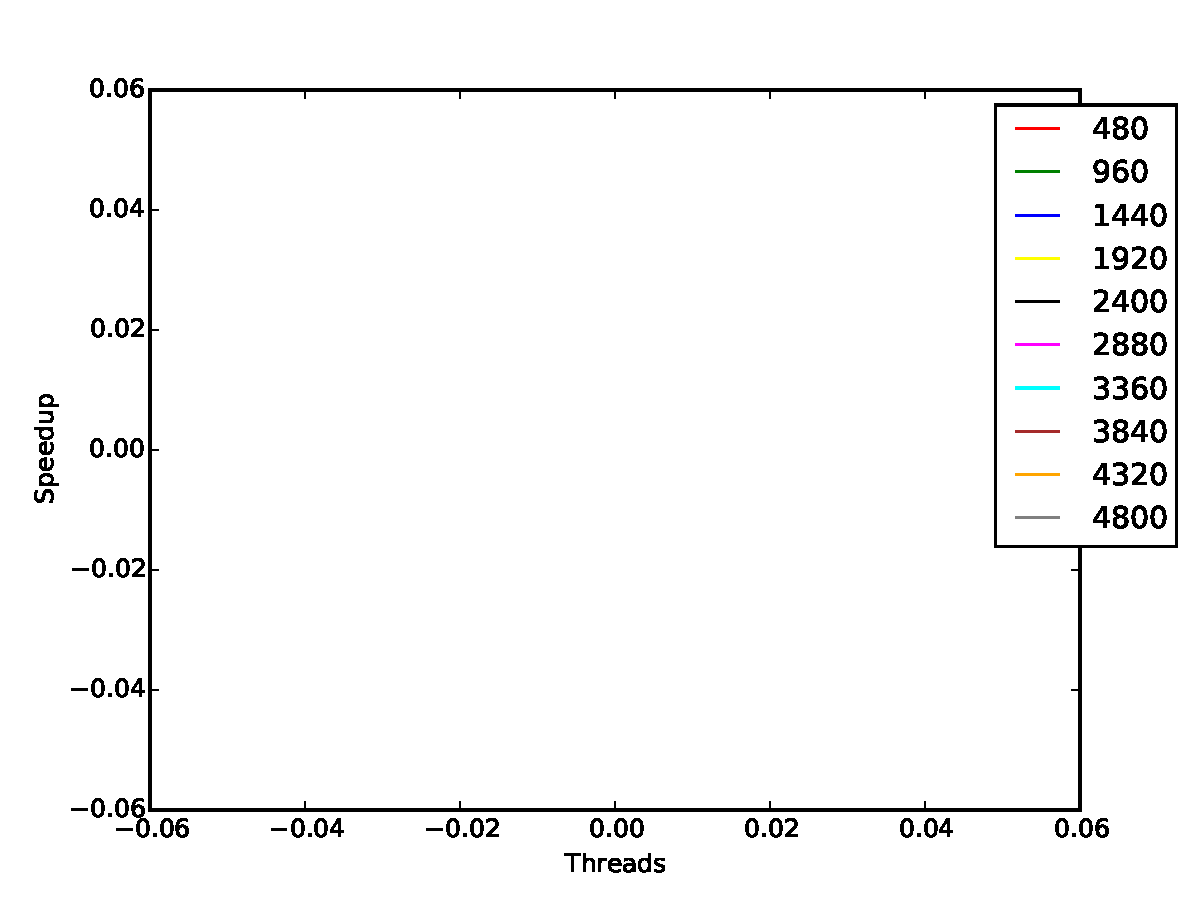
\includegraphics[width=0.5\textwidth]{plots/strong_fw-hybrid_baseline-fw-omp--1.pdf}
\caption{Strong scaling for fw-hybrid with a baseline of fw-omp}
\label{strong-fw-mpi}
\end{figure}

\section{Future Work}\label{sec:future}

\end{document}
